
\chapter{Modelo Macroscópico}
\label{cap:modeloMacroscopico}

En este capítulo veremos otro modelo matemático propuesto para el problema que vimos en la Sección \ref{cuestionAmodelizar}, donde exponíamos que una de las varias cuestiones que aún están por resolver en el mundo de la inmunología es qué mecanismos regulan la dinámica de población de las células T durante una respuesta inmune: una vez que las células se activan, ¿hasta cuándo continúan dividiéndose?, ¿es esta decisión totalmente dependiente de las condiciones que hayan tenido las células en el momento de su activación?, ¿por qué hay un retraso respecto a la desaparición del patógeno en la \textit{contracción clonal}?... 

En el Capítulo \ref{cap:descripcionTrabajo} se establece la base teórica de un modelo matemático a nivel microscópico, es decir, este modelo da el algoritmo de decisión para cada célula, pues las decisiones de las células inmunes son, \textit{a priori}, independientes, no se ha encontrado un órgano que las regule \citep{arias2016emergent}. Fue en el capítulo siguiente, el Capítulo \ref{cap:simulaciones}, donde vimos al modelo en acción, analizamos varias situaciones que podían modelarse, entre ellas las de tolerancia e intolerancia al \textit{patógeno}.

En este capítulo lo que haremos será volver a atajar este mismo problema pero desde una perspectiva un poco distinta, desde un punto de vista macroscópico. Esto quiere decir que las ecuaciones diferenciales sobre las que se basa el modelo servirán para modelar el comportamiento de toda la población como si de un único sistema se tratara. Para entender esto podemos poner como ejemplo un equipo de fútbol: la estrategia de contraataque del equipo vista desde el punto de vista <<macroscópico>> sería recuperar el balón y avanzar rápidamente al campo del adversario para marcar gol. Si nos fijamos ahora en el mundo <<microscópico>> de cada jugador, vemos que cada uno tiene su papel, defender y recuperar la posesión, pasar a los centrales o a los delanteros, etc. Ambos puntos de vista (macro y micro) dan lugar al mismo resultado y eso es justo lo que veremos en este capítulo, que las simulaciones del modelo macroscópico presentan el mismo aspecto que sus análogas del Capítulo \ref{cap:simulaciones}.

\section{Tolerancia y tasa de crecimiento}

La respuesta inmune adaptativa se basa en la capacidad que tienen las células T para identificar diferentes \textit{antígenos} pero ¿cómo saber cuáles de ellos son amigos y cuáles enemigos? En esta sección asumiremos que las células T toleran células cuyas tasas de crecimiento permanezcan por debajo de cierto límite, es decir, aquellas que no crezcan con mucha rapidez, las células que crecen muy rápidamente se asocian a toxinas o células tumorales, por ejemplo. Además, nos basaremos en dos características de la dinámica de población de las células T: la elasticidad (la población se expande y se contrae, lo conocemos como \textit{expansión} y \textit{contracción clonal}) y la inercia (la \textit{contracción clonal} se presenta con retraso tras la desaparición del \textit{patógeno}) \citep{arias2015growth}. Este resultado permite dar una posible explicación al hecho paradójico de que aquellos \textit{patógenos} que se desarrollan más lentamente en un organismo consigan sobrevivir o la presencia de células T autoreactivas PREGUNTAR QUÉ ES.


\section{Inercia y elasticidad en las células T}

Como ya hemos visto en la sección anterior, la inercia y elasticidad en la población de células T será el eje fundamental sobre el que se desarrolla el modelo macroscópico que se expone a continuación: 

Para empezar, nuestro modelo usa un sistema de ecuaciones diferenciales de segundo orden, estas son la manera más simple de representar la inercia de la población. Además, las ecuaciones de segundo grado son el marco general para las dinámicas \textit{newtonianas}. Esto nos lleva a modelar de manera natural la dinámica de las células T efectoras como el balance entre dos fuerzas opuestas actuando sobre la población: una fuerza por parte del \textit{antígeno} causada por la presencia del \textit{patógeno} y una fuerza intrínseca elástica que devuelve a la población a su estado inicial. En concreto, asumiremos que la fuerza que la fuerza que ejerce el \textit{antígeno} es proporcional al número de \textit{patógenos} y modelaremos la elasticidad mediante la Ley de Hook \citep{arias2015growth}, que establece que la fuerza necesaria para restablecer el equilibrio una vez que la población ha llegado a cierto valor, es proporcional a dicho valor. También asumiremos que el \textit{patógeno} prolifera con un ratio constante y que serán eliminados por la acción de las células T de manera proporcional a sus encuentros mutuos. De esta manera, presentamos el siguiente modelo:

\begin{equation}
	\label{sist_macro}
	\left\{ \begin{array}{l}
	{T^{\prime\prime}}(t) = -kT(t) + \lambda P(t) \\
	{P^{\prime}}(t) = \alpha P(t) - \beta T(t)P(t) \\
	\\
	T(0)=0 \hspace{3cm} ,para\, T \geq 0,\, P \geq P_m \\
	T^{\prime}(0)=0  \\
	P(0)=P_0 \geq P_m 6 \\ 
	\end{array}
	\right.
\end{equation}

Donde $T(t)$ y $P(t)$ son el número de células T efectoras y el número de células de \textit{patógeno}, respectivamente. A continuación veremos simulaciones de este modelo.

\section{Simulaciones del modelo macroscópico}


\begin{figure}[t]
	\centering
	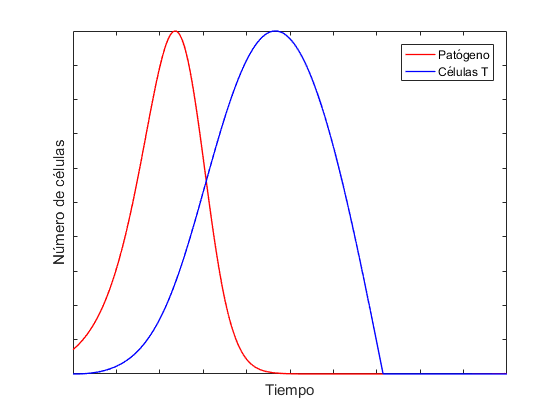
\includegraphics[width=0.7\textwidth]{Imagenes/Simulaciones/macro_intoler}
	\caption{Simulación: caso de intolerancia al patógeno en el modelo macroscópico.\\Parámetros: $\alpha=1,5$, $\beta=0,1$, $k=4$, $\lambda=0.5$}
	\label{fig:macro_intolerance}
\end{figure}

